\documentclass[letterpaper]{article}
\usepackage[utf8]{inputenc}
\usepackage[parfill]{parskip}    % Activate to begin paragraphs with an empty line rather than an indent
\usepackage{graphicx}
\usepackage{amssymb}
\usepackage{amsmath}
\usepackage{amsthm}
\usepackage{mathtools}

\usepackage{afterpage}

\usepackage{algorithm}
\usepackage{algpseudocode}

\usepackage{verse}

\newtheorem{theorem}{Theorem}[section]
\newtheorem{corollary}{Corollary}[theorem]
\newtheorem{lemma}[theorem]{Lemma}

\theoremstyle{remark}
\newtheorem*{remark}{Remark}

\usepackage{epstopdf}
\usepackage{circuitikz}
\usepackage[separate-uncertainty = true,multi-part-units=single]{siunitx}
\usepackage{booktabs}
\usepackage{enumitem}
\usepackage[toc,page]{appendix}
\usepackage{color}
\usepackage{pgfplots}
\usepackage{pgfplotstable}
\usepackage{caption}
\usepackage{subcaption}
\usepackage{url}
\usepackage{multirow}
\usepackage{makecell}
\usepackage[round]{natbib}   % omit 'round' option if you prefer square brackets
\usepackage{titling}
\usepackage{siunitx}

\usepackage{setspace}
% \doublespacing
\usepackage{float}


\pgfplotsset{compat=1.14}

%  Special math symbols
%       floor, ceiling, angled brackets
%-----------------------------------------------------------------------
\newcommand{\floor}[1]{\left\lfloor #1\right\rfloor}
\newcommand{\ceil}[1]{\left\lceil #1\right\rceil}
\newcommand{\etal}{\textit{et al.}}
\newcommand{\RE}{\mathbb{R}}        % real space
\newcommand{\ZZ}{\mathbb{Z}}        % integers
\newcommand{\NN}{\mathbb{N}}        % natural numbers
\newcommand{\eps}{{\varepsilon}}    % prettier epsilon
%-----------------------------------------------------------------------
%  Tighter lists
%-----------------------------------------------------------------------
\newenvironment{itemize*}% Tighter itemized list
  {\begin{itemize}%
    \setlength{\itemsep}{-0.5ex}%
    \setlength{\parsep}{0pt}}%
  {\end{itemize}}
\newenvironment{description*}% Tighter description list
  {\begin{description}%
    \setlength{\itemsep}{-0.5ex}%
    \setlength{\parsep}{0pt}}%
  {\end{description}}
\newenvironment{enumerate*}% Tighter enumerated list
  {\begin{enumerate}%
    \setlength{\itemsep}{-0.5ex}%
    \setlength{\parsep}{0pt}}%
  {\end{enumerate}}
%-----------------------------------------------------------------------
% Typing shortcuts
%-----------------------------------------------------------------------
\newcommand{\X}{\mathbb{X}}
\newcommand{\SG}{\mathbf{S}}
\newcommand{\GE}{\mathcal{G}}
\newcommand{\ST}{\,:\,}
\renewcommand{\tilde}[1]{\widetilde{#1}}
\newcommand{\diam}{\mathrm{diam}}
\newcommand{\sq}{\square}
\newcommand{\half}[1]{\frac{#1}{2}}
\newcommand{\inv}[1]{\frac{1}{#1}}
\newcommand{\alg}{\textsf{SplitReduce}}
\newcommand{\sz}[1]{\sigma_{#1}}
\newcommand{\LL}{\mathcal{L}}
\newcommand{\softOmega}{\widetilde{\Omega}} 
\newcommand{\softO}{\widetilde{O}}
\newcommand{\OO}{O^*}  %or \widetilde{O}?

\newcommand{\norm}[1]{\left\lVert#1\right\rVert}

\newcommand{\dx}{\mathrm{d}x}
\newcommand{\dy}{\mathrm{d}y}
\newcommand{\dz}{\mathrm{d}z}
\newcommand{\dt}{\mathrm{d}t}
\newcommand{\du}{\mathrm{d}u}
\newcommand{\dtheta}{\mathrm{d}\theta}
\newcommand{\dq}{\mathrm{d}q}
\newcommand{\diff}{\mathrm{d}}
\newcommand{\dV}{\mathrm{d}V}
\newcommand{\dL}{\mathrm{d}L}
\newcommand{\dA}{\mathrm{d}A}
\newcommand{\dH}{\mathrm{d}H}
\newcommand{\df}{\mathrm{d}f}
\newcommand{\dg}{\mathrm{d}g}
\newcommand{\dr}{\mathrm{d}r}
\newcommand{\dw}{\mathrm{d}w}
\newcommand{\dv}{\mathrm{d}v}
\newcommand{\dI}{\mathrm{d}I}

\newcommand*\len[1]{\overline{#1}}

\DeclarePairedDelimiter\abs{\lvert}{\rvert}%

\newcommand\note[1]{\marginpar{\textcolor{red}{#1}}}
\newcommand*{\tageq}{\refstepcounter{equation}\tag{\theequation}}

\newcommand*{\equals}{=}

\usepackage{fancyhdr}

\pgfplotscreateplotcyclelist{grayscale}{
    thick,white!10!black,mark=x,mark options=solid, dashed\\%
    thick,white!20!black,mark=o,mark options=solid\\%
}

\newcommand{\mat}[1]{\ensuremath{\begin{bmatrix}#1\end{bmatrix}}}
\newcommand{\eqn}[1]{\begin{alignat*}{2}#1\end{alignat*}}
\newcommand{\p}[2]{\frac{\partial #1}{\partial #2}}
\newcommand*{\thus}{&\implies\quad&}

\newcommand{\answer}[1]{\framebox{$\displaystyle #1 $}}

 
\pagestyle{fancy}
\fancyhf{}
\rhead{Rahul Arya}
\lhead{EE 16B}
\cfoot{\thepage}

\title{Lecture 5 - Notes}
\author{Rahul Arya}
\date{February 2019}
\begin{document}

\maketitle

\section{Overview}
Recall that frequency analysis focuses on analyzing the steady-state behavior of circuits with sinusoidal voltage and current sources.

A natural question to ask is: what's so special about sinusoids? One aspect is that sinusoid sources are very common - for instance, in the voltage output by a dynamo - making this form of analysis very useful. In addition, it turns out that through an algorithm known as the \emph{discrete Fourier transform}, any periodic input signal can be decomposed into a sum of sinusoidal functions. The most important reason, however, is that analyzing sinusoidal functions is \emph{easy}! Whereas analyzing arbitrary input signals (like in transient analysis) requires us to solve a set of differential equations, it turns out that we can use a procedure very similar to the seven-step procedure from EE16A in order to solve AC circuits with only sinusoidal sources.

\section{Sinusoids}
First, though, we will establish some terminology. Consider the function $X(t) = A\sin{\omega t}$:
\begin{center}
\begin{tikzpicture}
\begin{axis}[
    xmin=0, xmax=10,
    ymin=-1.5, ymax=1.5,
    axis lines=middle,
    xlabel=$t$,
]
\addplot[mark=none, samples=200, domain=0:10] {sin(x * 180 / pi)};
\addlegendentry{$X(t)$}
\end{axis}
\end{tikzpicture}
\end{center}
You can think of $X$ as representing an alternating current or voltage. We call the maximum value of $X$ above the mean (in this case, the $x$-axis) the \emph{amplitude} ($A$), and the spacing between repetitions of the function the \emph{period} ($T$ = $2\pi / \omega$). We considered these properties of sinusoids in the previous lecture, when discussing the impedance magnitude. However, there is one final property of sinusoids: their \emph{phase}. Consider the function $Y(t) = A\sin{\omega t + \phi}$:
\begin{center}
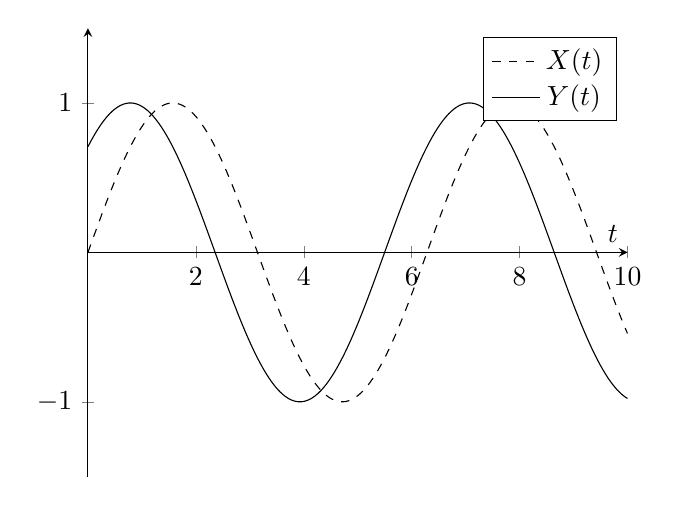
\begin{tikzpicture}
\begin{axis}[
    xmin=0, xmax=10,
    ymin=-1.5, ymax=1.5,
    axis lines=middle,
    xlabel=$t$,
]
\addplot[mark=none, dashed, samples=200, domain=0:10] {sin(x * 180 / pi)};
\addplot[mark=none, samples=200, domain=0:10] {sin(x * 180 / pi + 45)};
\addlegendentry{$X(t)$}
\addlegendentry{$Y(t)$}
\end{axis}
\end{tikzpicture}
\end{center}
Here, $\phi$ represents the \emph{phase shift} of $Y$ with respect to $X$. As can be seen, a positive phase shift moves the function to the left by that amount. In particular, notice that the sine and cosine functions are really the same sinusoid, with each just the other after a $\pi/2$ radian phase shift in the appropriate direction.

\section{Phase Shifts and Phasors}
Now, we will consider the behavior of capacitors and inductors when supplied with a sinusoidal voltage. First, let's look at a capacitor provided with the sinusoidal voltage $V(t) = V_0\cos{\omega t}$, as shown:
\begin{center}
\begin{circuitikz}[american]
\draw (0, 0) node[ocirc]{} to[C, l=$C$, v=$V_0\cos{\omega t}$, i=$I(t)$] (2, 0) node[ocirc]{};
\end{circuitikz}
\end{center}
Note that we aren't assuming anything about the origin of the $V(t)$ - it could come from a voltage supply directly, or from some other complicated circuit.

From the capacitor equation, and applying basic calculus, we find that
\eqn{
    && I(t) &= C \frac{\diff V}{\dt} \\
    &&&= -\omega C V_0 \sin{\omega t}.
}
Ideally, we'd like to obtain some sort of linear relationship between $V(t)$ and $I(t)$, similar to the resistance of a resistor. However, here we find that
\[
    \frac{V(t)}{I(t)} = -\frac{1}{\omega C} \cot{\omega t},
\]
which doesn't seem very useful, since it varies with time, taking on all the values from $-\infty$ to $\infty$.

The key issue here is the phase shift from $\cos{\omega t}$ to $\sin{\omega t}$, which messes up our attempt to calculate a ratio. It would be nice if we could rewrite our sinusoids in a manner where we could calculate some sort of ratio of sinusoids of different phases that remained invariant with time, as then we'd be able to get some sort of reasonable analogue of resistance.

To do this, we will use complex numbers. These notes assume a basic understanding of complex numbers, at the level of the following properties, presented without further elaboration:
\eqn{
    && j^2 &= -1 \\
    && (a + bj) (c + dj) &= (ac - bd) + (bc + ad)j \\
    && (a + bj) + (c + dj) &= (a + c) + (b + d)j \\
    && \overline{a + bj} &= a - bj \\
    && z\overline{z} &= \abs{z}^2 \in \mathbb{R}.
}
If any of these properties or any of the notation are unfamiliar, please refer to the first few sections of the course notes on complex numbers\footnote{In mathematics, you may have seen $i$ used to denote $\sqrt{-1}$. In electrical engineering, we use $j$, to avoid confusing it with the use of the letter $i$ for current. The underlying principles, of course, are exactly the same no matter which letter you use!}.

There is one more, less trivial, result about complex numbers, known as \emph{Euler's formula}, that is important. The proof of this equation is not required for our circuit analysis, but is provided in the course notes on complex numbers. The formula itself states that, for any real angle $\theta$,
\[
    e^{j\theta} = \cos{\theta} + j\sin{\theta}.
\]
From this equation, and basic algebraic manipulation, we immediately see that
\eqn{
    && \cos{\theta} &= \frac{(\cos{\theta} + j\sin{\theta}) + (\cos{\theta} - j\sin{\theta})}{2} \\
    &&&= \frac{e^{j\theta} + e^{-j\theta}}{2} \\
    && \sin{\theta} &= \frac{(\cos{\theta} + j\sin{\theta}) - (\cos{\theta} - j\sin{\theta})}{2j} \\
    &&&= \frac{e^{j\theta} - e^{-j\theta}}{2j}.
}
Also note that
\eqn{
    && \overline{e^{j\theta}} &= \overline{\cos{\theta} + j\sin{\theta}} \\
    &&&= \cos{\theta} - j\sin{\theta} \\
    &&&= \cos{(-\theta)} + j\sin{(-\theta)} \\
    &&&= e^{-j\theta}.
}

Now, let's return to our analysis of the capacitor. Rewriting our results using these new forms of sinusoids, we find that
\eqn{
    && V(t) &= V_0\cos{\omega t} \\
    &&&= \frac{V_0}{2} e^{j\omega t} + \frac{V_0}{2} e^{-j\omega t} \\
    &&&= \frac{1}{2} \left( V_0 e^{j\omega t} + \overline{V_0} e^{-j\omega t} \right) \\
    && I(t) &= -\omega C V_0 \sin{\omega t} \\
    &&&= -\frac{\omega C V_0}{2j} (e^{j\omega t} - e^{-j\omega t}) \\
    &&&= \frac{j\omega C V_0}{2} e^{j\omega t} + (-\frac{j\omega C V_0}{2}) e^{-j\omega t} \\
    &&&= \frac{1}{2} \left(j \omega C V_0 e^{j\omega t} + \overline{j \omega C V_0} e^{-j\omega t} \right)
}

Notice now how $V(t)$ and $I(t)$ have very similar forms - that of
\[
    f(t) = \frac{1}{2} \left(\tilde{X}e^{j\omega t} + \overline{\tilde{X}} e^{-j\omega t} \right),
\]
where $\tilde{X}$ is some complex number that does not depend on $t$. We call $\tilde{X}$ a \emph{phasor} representing $f(t)$. Thus, here we have the phasors $\tilde{V}$ and $\tilde{I}$ representing the voltage and current across the capacitor to be
\eqn{
    && \tilde{V} &= V_0 \\
    && \tilde{I} &= j\omega C V_0.
}
We define the \emph{impedance} $\tilde{Z}$ of a capacitor to be
\[
    \tilde{Z} = \frac{\tilde{V}}{\tilde{I}} = \frac{1}{j\omega C}.
\]
It should be clear, though we have not proven it here formally, that $\tilde{Z}$ will be the same no matter what input voltage $V(t)$ we supply, so long as it can be represented by some phasor $\tilde{V}$ (like all sinusoids can). Also, observe that the amplitude of any sinusoidal function equals the absolute value of its corresponding phasor, and its phase shift is its phasor's argument.

\section{Impedance of Circuit Elements}
We will now quickly perform a similar analysis for inductors and resistors.

Imagine some resistor $R$ as follows:
\begin{center}
\begin{circuitikz}[american]
\draw (0, 0) node[ocirc]{} to[R, l=$R$, v=$V(t)$, i=$I(t)$] (2, 0) node[ocirc]{};
\end{circuitikz}
\end{center}
Let $V(t)$ be represented by some phasor $\tilde{V}$. Thus, by Ohm's Law,
\eqn{
    && V(t) &= \frac{1}{2} \left(\tilde{V} e^{j\omega t} + \overline{\tilde{V}} e^{-j\omega t} \right) \\
    \thus I(t) &= \frac{1}{R} V(t) \\
    &&&= \frac{1}{2} \left(\frac{\tilde{V}}{R} e^{j\omega t} + \overline{\frac{\tilde{V}}{R}} e^{-j\omega t} \right),
}
so we may represent the output current with the phasor
\[
    \tilde{I} = \frac{\tilde{V}}{R},
\]
so the impedance is clearly
\[
    \tilde{Z} = R.
\]
From this, we see that the impedance behaves very much like the resistance does, except that it generalizes to other circuit components.

Now, we will consider inductors. It should be clear that any sinusoidal function can be represented by a phasor (though this still requires a proof!). Thus, since a sinusoidal voltage will always lead to a sinusoidal current through an inductor, we can start with a sinusoidal current and work in the opposite direction to calculate the impedance of an inductor, as follows.

Consider an inductor with voltage and current across it as follows:
\begin{center}
\begin{circuitikz}[american]
\draw (0, 0) node[ocirc]{} to[L, l=$L$, v=$V(t)$, i=$I(t)$] (2, 0) node[ocirc]{};
\end{circuitikz}
\end{center}
Let the current $I(t)$ be represented by some phasor $\tilde{I}$. Thus, by the equation of an inductor,
\eqn{
    && I(t) &= \frac{1}{2} \left(\tilde{I} e^{j\omega t} + \overline{\tilde{I}} e^{-j\omega t} \right) \\
    \thus V(t) &= L \frac{\dI}{\dt} \\
    &&&= \frac{1}{2} \left(j\omega L\tilde{I} - j \omega L\overline{I} e^{-j \omega t} \right) \\
    &&&= \frac{1}{2} \left( j\omega L\tilde{I} + \overline{j\omega L \tilde{I}} e^{-j \omega t} \right),
}
so the voltage can be represented by the phasor
\[
    \tilde{V} = j\omega L\tilde{I}.
\]
Thus, the impedance of an inductor is
\[
    \tilde{Z} = j\omega L.
\]

\section{Circuit Analysis}
At this point, observe that we have essentially obtained ``equivalents'' to Ohm's Law for inductors and capacitors, using the impedance to relate their voltage and current phasors. Note also that, for a sum of sinusoidal functions to be zero, the sum of the phasors of each of those functions must equal zero as well. This result can be thought of as a generalization of KCL to phasors.

Putting everything together, we have now successfully generalized all of our techniques of DC analysis to frequency analysis. We can finally generalize some basic circuits, to verify that our technique works correctly.

Consider a voltage divider, where instead of one resistor we introduce a capacitor, as follows:
\begin{center}
\begin{circuitikz}[american]
\draw (0, 0) node[ground] {} to[sinusoidal voltage source, l=$V_0\cos{\omega t}$, v<=$ $] (0, 4) to (2, 4) to[C, l=$C$] (2, 2) node[ocirc] {} node[right] {$u(t)$} to[R, l=$R$] (2, 0) to (0, 0);
\end{circuitikz}
\end{center}
We are interested in knowing how the voltage $u(t)$ varies over time. Recall that we proved the voltage divider equation in the context of DC circuit analysis. However, that proof carries over to frequency analysis in a straightforward manner. Thus, the phasor $\tilde{u}$ representing the voltage $u(t)$ can be represented in terms of the phasor $\tilde{V}$ representing the supply voltage as follows:
\[
    \tilde{u} = \frac{Z_R}{Z_C + Z_R} \tilde{V},
\]
where $Z_C$ and $Z_R$ are the impedances of the capacitor and resistor, respectively. Note also that, since the supply is at frequency $\omega$, all other voltages and currents in the system will also be at the same frequency $\omega$. Thus, using our results from earlier, we know that
\[
    Z_C = \frac{1}{j\omega C}
\]
and
\[
    Z_R = R.
\]
Note also that $\tilde{V} = V_0$, using our equation for $\cos{\theta}$ from earlier.

Substituting these values into our equation for $\tilde{u}$, we find that
\[
    \tilde{u} = \frac{R}{\frac{1}{j\omega C} + R} V_0,
\]
which allows us to solve for $u(t)$ exactly (using the equation converting phasors back into real-valued functions).

\end{document}
